\chapter{日地系统的数值模拟}

\section{从相对运动系开始的数值模拟框架}

由第一章可知，日地系统在质心系中的内部动力学由
\[
\ddot{\bm r}=-\mu \frac{\bm r}{\|\bm r\|^3},
\qquad
\mu=G(M_S+M_E)
\]
决定，其中 \(\bm r=\bm r_E-\bm r_S\) 表示地球相对太阳的位置向量。
数值模拟时，不必直接积分 \(\bm r_S,\bm r_E\) 两组耦合方程，而是先积分 \(\bm r\)，再由
\[
\bm r_S=-\frac{M_E}{M_S+M_E}\bm r,
\qquad
\bm r_E=\frac{M_S}{M_S+M_E}\bm r
\]
恢复太阳和地球在质心系中的位置\cite{MurrayDermott1999,BateMuellerWhite1971}。

这种做法的优点是：
\begin{enumerate}[label=\arabic*.]
  \item 消除了不必要的整体平移自由度；
  \item 直接抓住了引力作用依赖的相对位置；
  \item 更便于讨论能量、角动量与轨道几何；
  \item 便于将二维模型推广到三维模型。
\end{enumerate}

\section{二维模型与无量纲化}

若先在固定平面内模拟，例如取 \(xy\)-平面，则令
\[
\bm r(t)=(x(t),y(t)).
\]
方程化为\cite{BateMuellerWhite1971}
\begin{equation}\label{eq:2d-second}
\ddot x=-\mu \frac{x}{(x^2+y^2)^{3/2}},
\qquad
\ddot y=-\mu \frac{y}{(x^2+y^2)^{3/2}}.
\end{equation}

令
\[
v_x=\dot x,\qquad v_y=\dot y,
\]
则可写成一阶系统
\begin{equation}\label{eq:2d-first}
\dot x=v_x,\qquad \dot y=v_y,
\end{equation}
\begin{equation}\label{eq:2d-first-2}
\dot v_x=-\mu \frac{x}{(x^2+y^2)^{3/2}},
\qquad
\dot v_y=-\mu \frac{y}{(x^2+y^2)^{3/2}}.
\end{equation}

为简化数值实验，下面先使用无量纲单位：
\begin{itemize}
  \item 长度单位取 \(1\,\mathrm{AU}\)；
  \item 时间单位取 \(1\,\mathrm{year}\)；
  \item 令地球平均轨道半径近似为 \(1\)；
  \item 令地球绕太阳一周的周期近似为 \(1\)。
\end{itemize}
在此单位制下，圆轨道条件给出
\[
\mu=4\pi^2.
\]
这时圆轨道的一个标准初值为
\begin{equation}\label{eq:circular-ic}
x(0)=1,\qquad y(0)=0,\qquad v_x(0)=0,\qquad v_y(0)=2\pi.
\end{equation}
理论解为
\[
x(t)=\cos(2\pi t),\qquad y(t)=\sin(2\pi t).
\]

\begin{figure}[htbp]
\centering
\begin{tikzpicture}[scale=3]

  % 坐标轴
  \draw[->, thin] (-1.3,0) -- (1.35,0) node[below right] {$x$};
  \draw[->, thin] (0,-1.3) -- (0,1.35) node[left] {$y$};

  % 单位圆轨道
  \draw[thick, blue] (0,0) circle (1);

  % 太阳
  \filldraw[orange] (0,0) circle (0.035);
  \node[below right] at (0,0) [orange]{太阳};

  % 初始点
  \filldraw[blue] (1,0) circle (0.03);
  \node[below right] at (1,0) {$\bigl(1,0\bigr)$};

  % 初速度箭头
  \draw[->, very thick, blue] (1,0) -- (1,0.45);
  \node[right] at (1,0.48) [blue]{$\bm v(0)=(0,2\pi)$};

  % 轨道方向箭头
  \draw[->, thick, blue] (0.55,0.84) arc[start angle=57,end angle=77,radius=1];

  % 单位圆标注
  \node[blue] at (-0.7,1.00) {$x^2+y^2=1$};

  % 原点标注
  \node[below left] at (0,0) {$O$};

  % 地球标注
  \node[above right] at (1,0) [blue]{地球};


\end{tikzpicture}
\caption{二维无量纲模型下的圆轨道初值示意图。地球初始位置取为 \((1,0)\)，初始速度竖直向上，
故轨道为逆时针方向的单位圆。}
\label{fig:circular-ic}
\end{figure}

由初值
\[
x(0)=1,\qquad y(0)=0,\qquad v_x(0)=0,\qquad v_y(0)=2\pi,
\]
可知轨道从点 \((1,0)\) 出发，并沿逆时针方向绕单位圆运动，这与理论解
\[
x(t)=\cos(2\pi t),\qquad y(t)=\sin(2\pi t)
\]
完全一致。

\section{Euler 方法的原理与应用}

\subsection{Euler 方法的基本思想}

Euler 方法来源于最简单的一阶 Taylor 截断\cite{HairerLubichWanner2006,LeimkuhlerReich2004}。对一阶系统
\[
\dot Y=f(Y)
\]
在时刻 \(t_n\) 处作展开，得到
\[
Y(t_{n+1})=Y(t_n)+h f(Y(t_n))+O(h^2),
\]
其中 \(h=t_{n+1}-t_n\) 为时间步长。因此，舍去高阶项后得到显式 Euler 格式
\begin{equation}\label{eq:euler-general}
Y_{n+1}=Y_n+h f(Y_n).
\end{equation}

将 \eqref{eq:2d-first}--\eqref{eq:2d-first-2} 视为一阶系统，状态向量取为
\[
Y=(x,y,v_x,v_y)^\top,
\]
则 Euler 方法的迭代公式为
\begin{align}
 x_{n+1} &= x_n+h v_{x,n},\label{eq:euler-x}\\
 y_{n+1} &= y_n+h v_{y,n},\label{eq:euler-y}\\
 v_{x,n+1} &= v_{x,n}-h\mu \frac{x_n}{(x_n^2+y_n^2)^{3/2}},\label{eq:euler-vx}\\
 v_{y,n+1} &= v_{y,n}-h\mu \frac{y_n}{(x_n^2+y_n^2)^{3/2}}.\label{eq:euler-vy}
\end{align}

\subsection{Euler 方法在轨道问题中的特点}

Euler 方法的优点是公式极其简单，适合入门、调试和作为对照实验；但在轨道问题中，它有明显缺点：
\begin{enumerate}[label=\arabic*.]
  \item 它只有一阶精度，步长稍大时误差积累很快；
  \item 它不保持哈密顿系统的几何结构（圆形轨道在长期积分中会逐渐变形）；
  \item 在长期传播中，能量往往出现明显漂移（能量不守恒）；
  \item 对周期轨道，常见现象是轨道逐渐向外发散或向内坍缩。
\end{enumerate}
因此，Euler 方法更适合用来说明“一个不适合轨道长期传播的方法会出现什么问题”，而不适合作为正式的轨道长期模拟方法。

\section{Velocity-Verlet 方法的原理与应用}

\subsection{从二阶系统出发}

对于形如
\[
\ddot{\bm r}=\bm a(\bm r)
\]
的二阶系统，其中加速度仅依赖于位置，Velocity-Verlet 是最自然的时间离散格式之一。对于日地相对运动，有
\[
\bm a(\bm r)=-\mu \frac{\bm r}{\|\bm r\|^3}.
\]

\subsection{从 Taylor 展开导出位置更新}

对位置作 Taylor 展开：
\[
\bm r(t+h)=\bm r(t)+h\bm v(t)+\frac{h^2}{2}\bm a(t)+O(h^3).
\]
因此可用
\begin{equation}\label{eq:vv-r}
\bm r_{n+1}=\bm r_n+h\bm v_n+\frac{h^2}{2}\bm a_n
\end{equation}
更新位置，其中 \(\bm a_n=\bm a(\bm r_n)\)。

在得到 \(\bm r_{n+1}\) 后，计算新位置对应的加速度
\[
\bm a_{n+1}=\bm a(\bm r_{n+1}).
\]
然后利用当前与下一步加速度的平均值更新速度：
\begin{equation}\label{eq:vv-v}
\bm v_{n+1}=\bm v_n+\frac{h}{2}(\bm a_n+\bm a_{n+1}).
\end{equation}
这就是 Velocity-Verlet 的基本格式。

\subsection{哈密顿观点下的解释}

对于可分离哈密顿系统
\[
H(q,p)=T(p)+V(q),
\]
Velocity-Verlet 也可视为一种 ``kick--drift--kick'' 的对称分裂：
\[
p^{n+\frac12}=p^n-\frac{h}{2}\nabla V(q^n),
\]
\[
q^{n+1}=q^n+h\,p^{n+\frac12},
\]
\[
p^{n+1}=p^{n+\frac12}-\frac{h}{2}\nabla V(q^{n+1}).
\]
因此，对固定步长的可分离保守系统，Velocity-Verlet 是一个二阶、时间可逆、保辛的积分格式。它一般并不在每一步严格守恒原始能量，但常见现象是：长期积分中能量误差呈有界振荡，而不是像 Euler 方法那样持续漂移。

\subsection{二维情形下的具体实现}

对二维状态 \(\bm r_n=(x_n,y_n)\)、\(\bm v_n=(v_{x,n},v_{y,n})\)，加速度函数为
\[
\bm a(\bm r)=
-\mu \frac{\bm r}{\|\bm r\|^3}
=
\left(
-\mu \frac{x}{(x^2+y^2)^{3/2}},
-\mu \frac{y}{(x^2+y^2)^{3/2}}
\right).
\]
因此每一步迭代为
\[
\bm a_n=\bm a(\bm r_n),
\]
\[
\bm r_{n+1}=\bm r_n+h\bm v_n+\frac{h^2}{2}\bm a_n,
\]
\[
\bm a_{n+1}=\bm a(\bm r_{n+1}),
\]
\[
\bm v_{n+1}=\bm v_n+\frac{h}{2}(\bm a_n+\bm a_{n+1}).
\]

\section{圆轨道上 Euler 与 Velocity-Verlet 的对比实验}

\subsection{实验设置}

为了直接比较两种方法，考虑圆轨道初值 \eqref{eq:circular-ic}，模拟一整年（即一个完整周期），比较：
\begin{enumerate}[label=\arabic*.]
  \item 一周后终点与理论点 \((1,0)\) 的位置误差；
  \item 相对能量误差 \( |E_N-E_0|/|E_0| \)；
  \item 相对角动量误差 \( |L_N-L_0|/|L_0| \)。
\end{enumerate}
其中
\[
E=\frac12(v_x^2+v_y^2)-\frac{\mu}{\sqrt{x^2+y^2}},
\qquad
L=xv_y-yv_x.
\]

\subsection{一个具体数值例子}

取两组典型步长 \(h=10^{-2}\) 与 \(h=10^{-3}\)，数值实验结果可整理为表 \ref{tab:euler-vv-circle}。

\begin{table}[H]
\centering
\caption{圆轨道上一周期后 Euler 与 Velocity-Verlet 的对比}
\label{tab:euler-vv-circle}
\begin{tabular}{cccccc}
\toprule
方法 & 步长 \(h\) & 位置误差 & 相对能量误差 & 相对角动量误差 & 现象 \\
\midrule
Euler & $10^{-2}$ & $2.2556$ & $3.4845\times 10^{-1}$ & $2.2650\times 10^{-1}$ & 轨道明显发散 \\
Velocity-Verlet & $10^{-2}$ & $8.2560\times 10^{-3}$ & $4.2229\times 10^{-12}$ & $1.4136\times 10^{-16}$ & 仍接近圆轨道 \\
Euler & $10^{-3}$ & $3.5853\times 10^{-1}$ & $6.8360\times 10^{-2}$ & $3.6033\times 10^{-2}$ & 漂移仍明显 \\
Velocity-Verlet & $10^{-3}$ & $8.2682\times 10^{-5}$ & $5.3995\times 10^{-15}$ & $2.6858\times 10^{-15}$ & 结果极稳定 \\
\bottomrule
\end{tabular}
\end{table}

\begin{figure}[H]
\centering
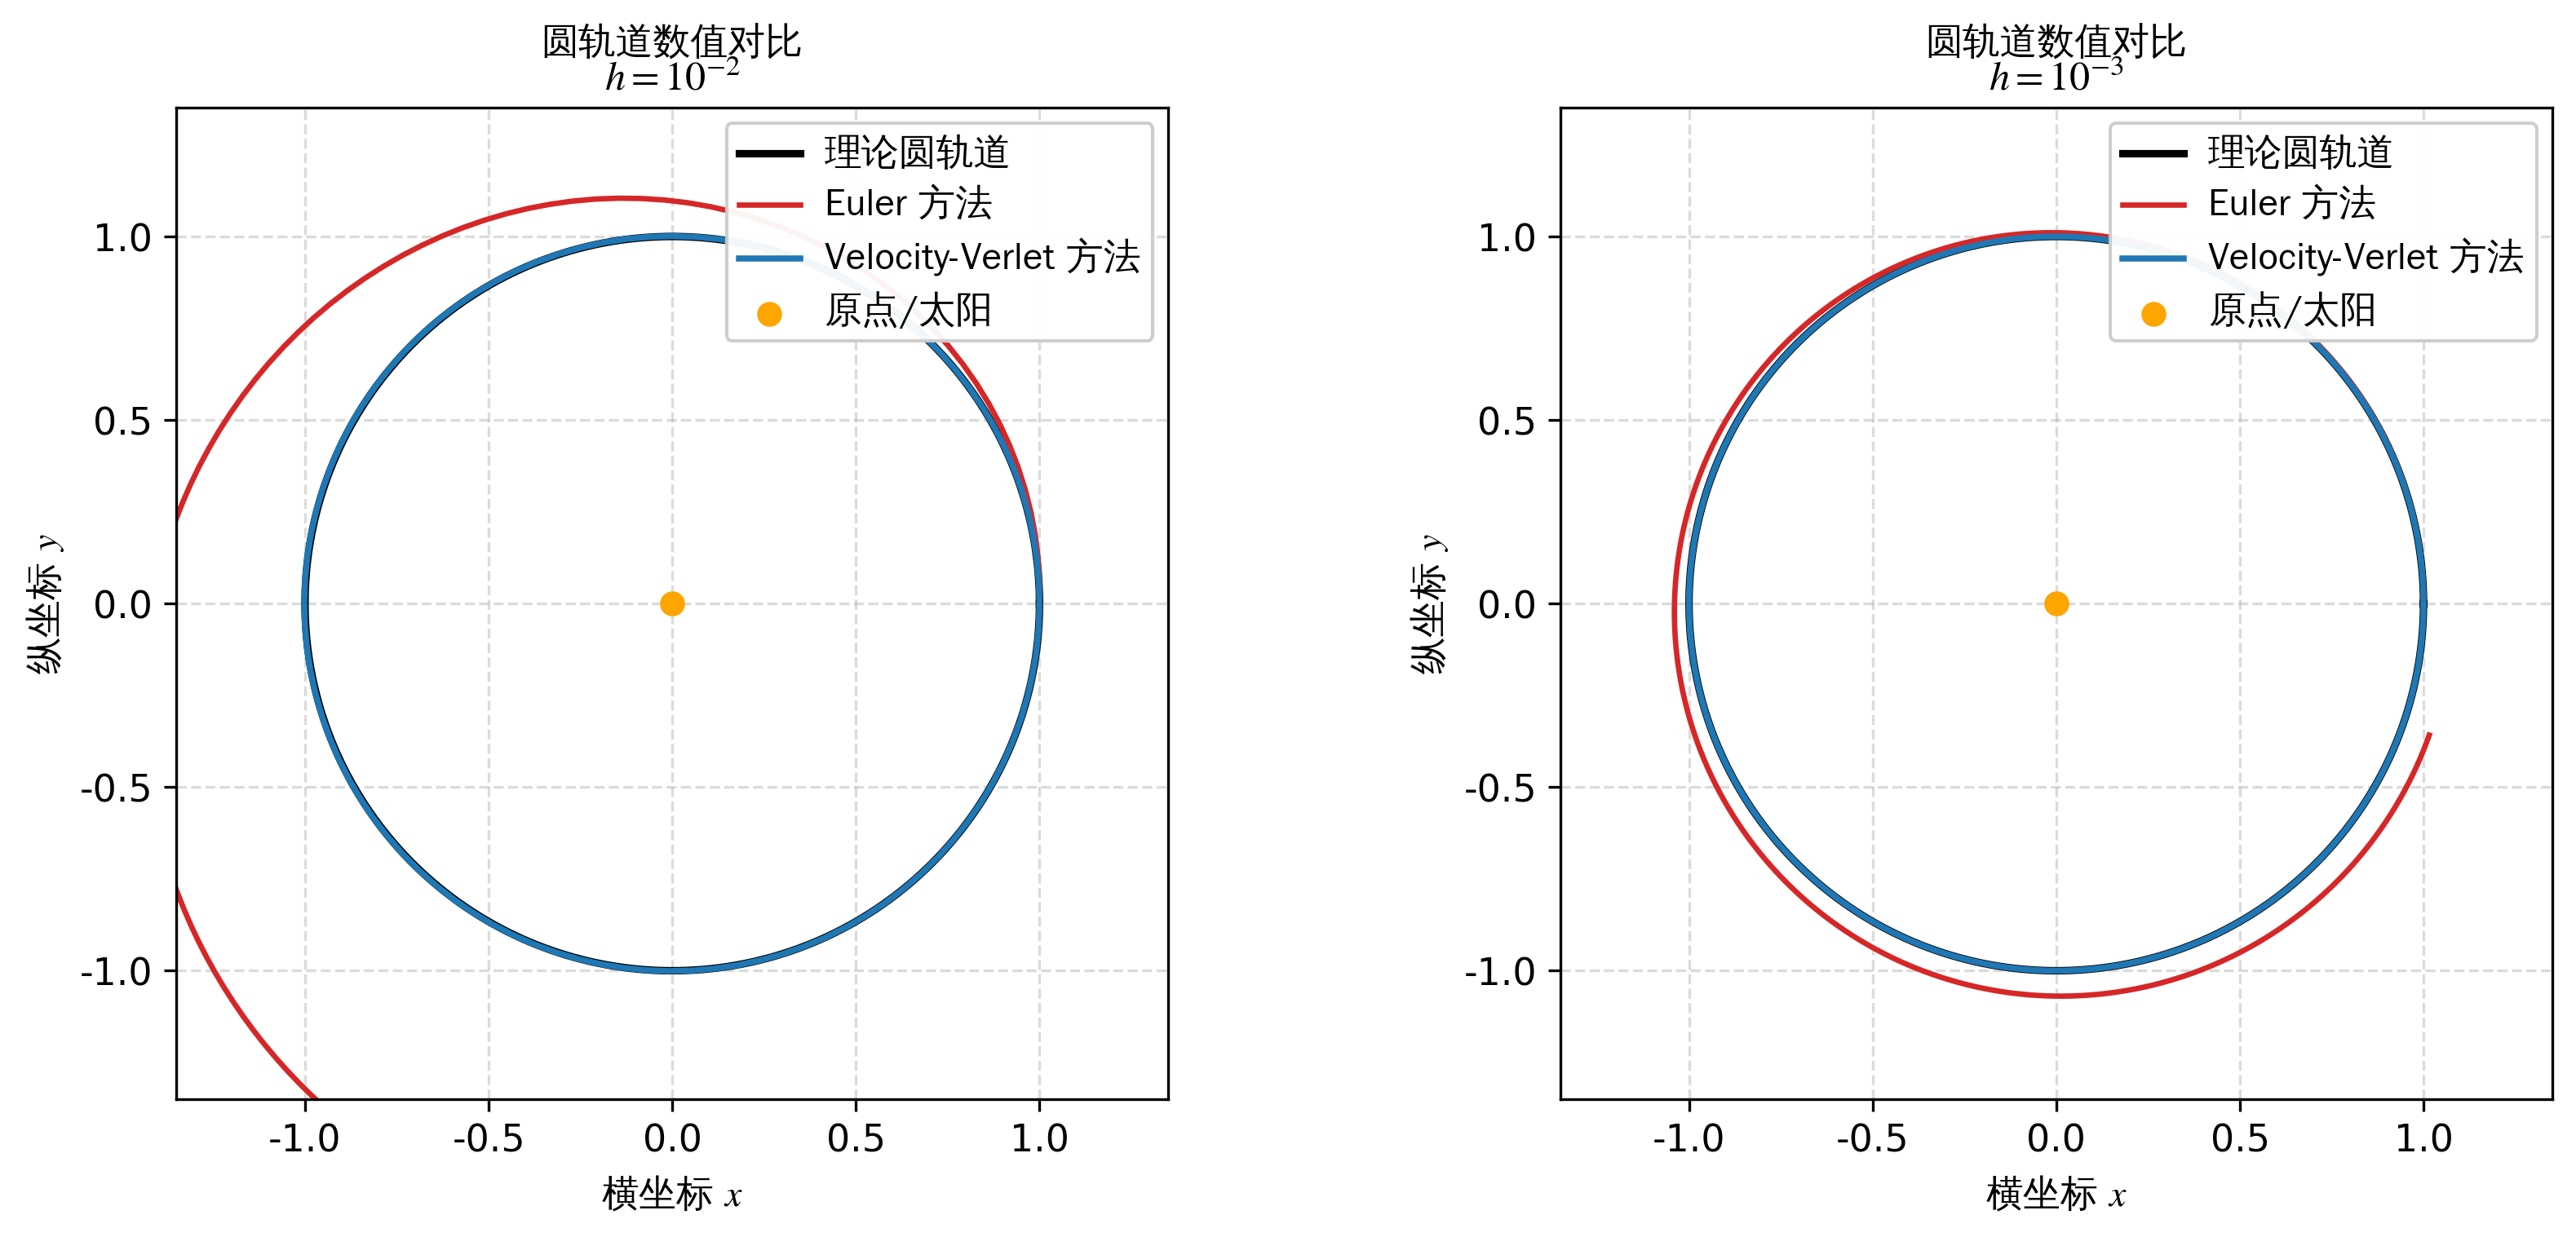
\includegraphics[width=0.92\textwidth]{images/circle_orbit_comparison.png}
\caption{圆轨道上一周期内的数值轨道对比。左图对应步长 \(h=10^{-2}\)，右图对应步长 \(h=10^{-3}\)。黑色曲线为理论圆轨道，红色曲线为 Euler 方法得到的数值轨道，蓝色曲线为 Velocity-Verlet 方法得到的数值轨道，橙色点表示原点处的太阳。可以看到，当步长较大时，Euler 方法出现明显轨道漂移，而 Velocity-Verlet 方法仍能较好保持圆轨道结构；当步长减小到 \(10^{-3}\) 时，两者误差均减小，但 Velocity-Verlet 方法仍明显更稳定。}
\label{fig:circle-orbit-comparison}
\end{figure}

\begin{figure}[H]
\centering
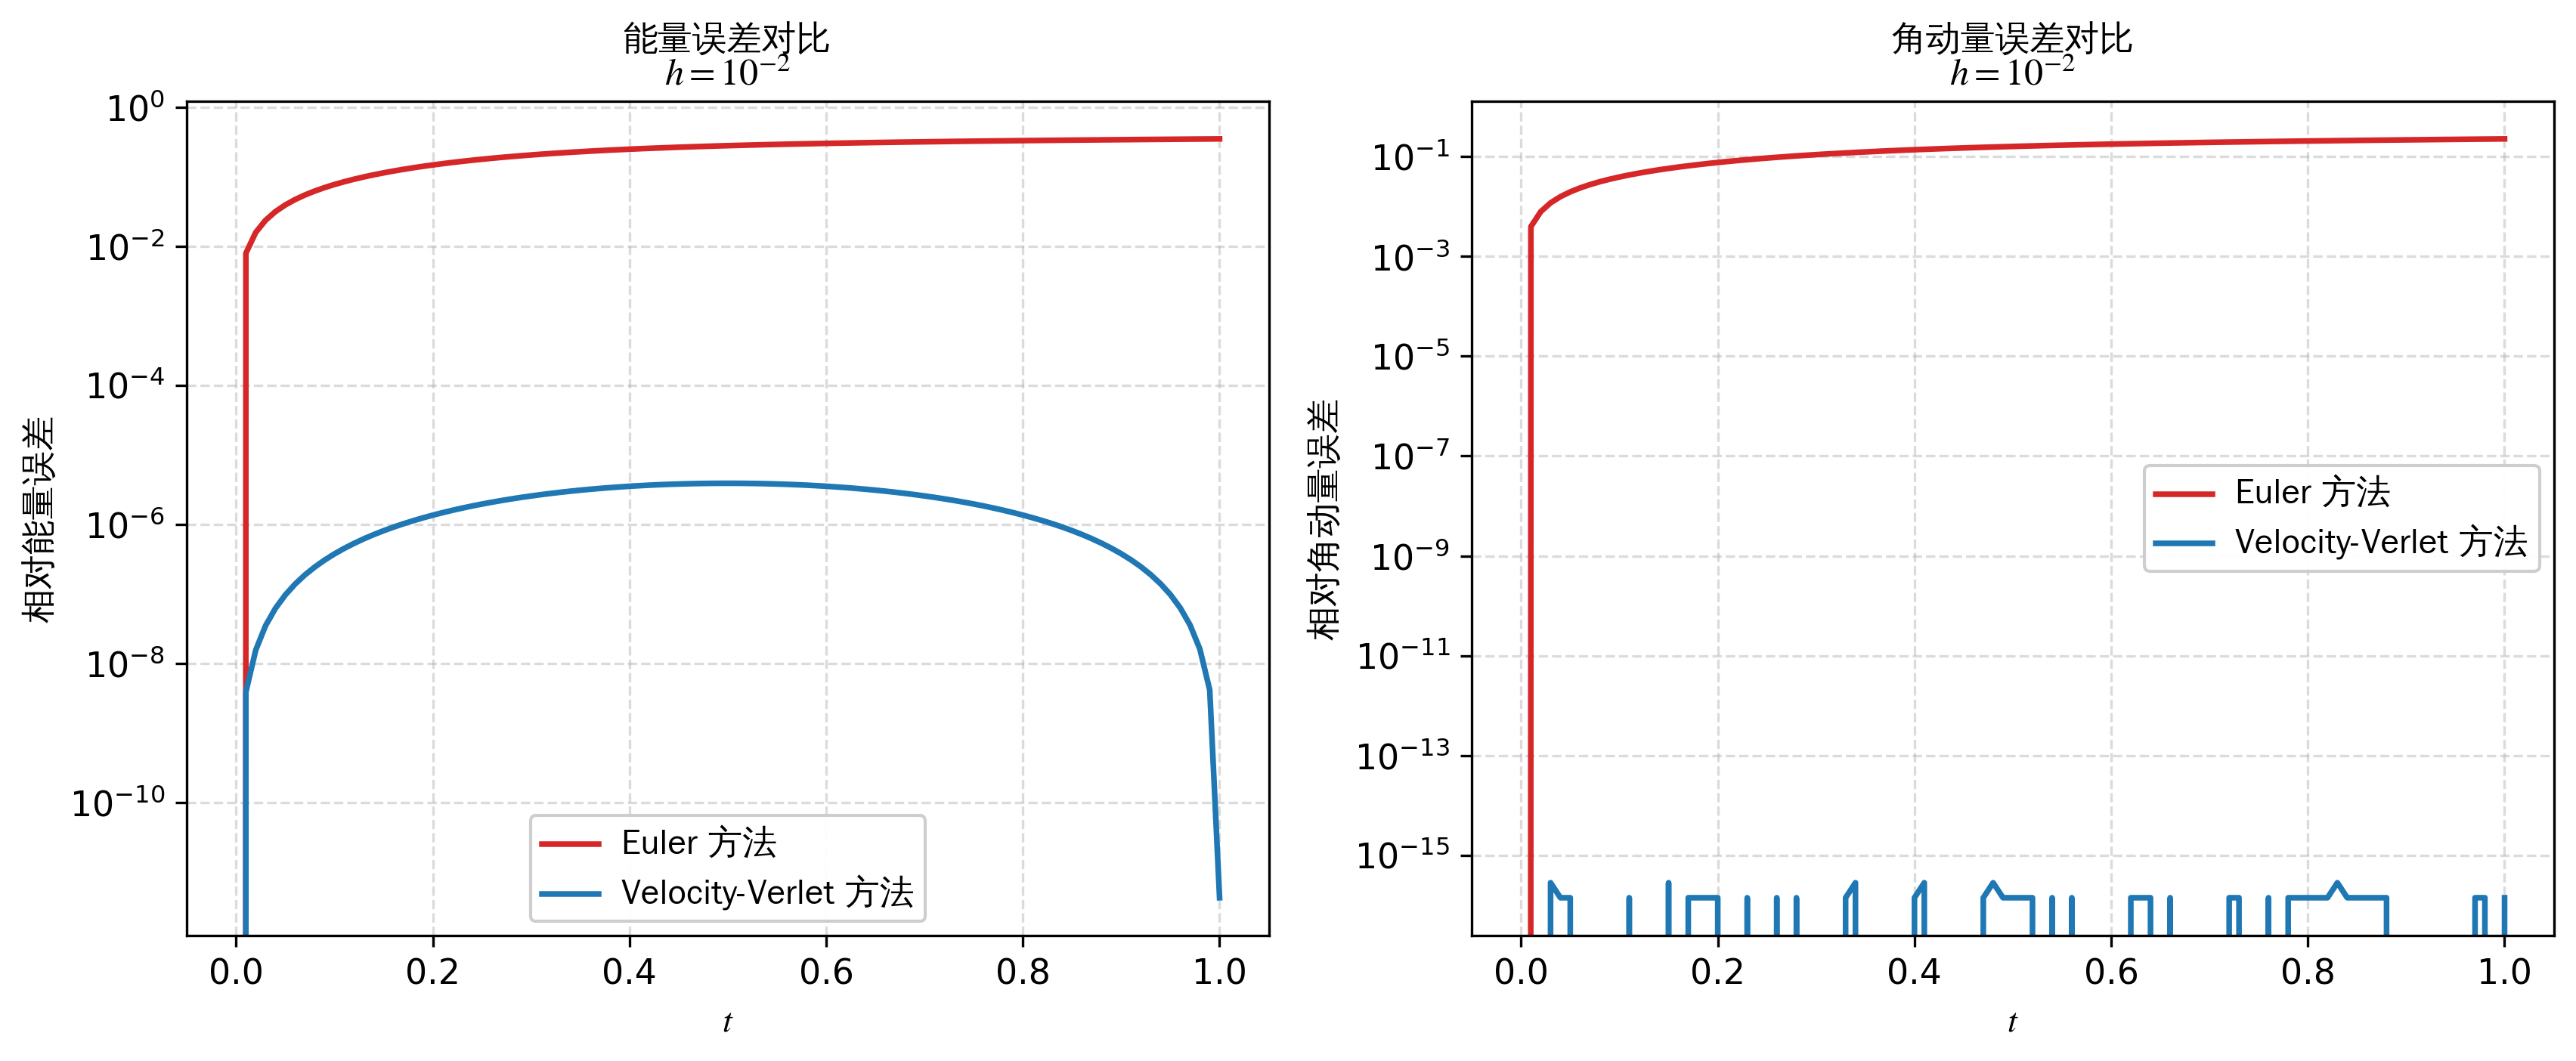
\includegraphics[width=0.92\textwidth]{images/conservation_errors_h1e-02.png}
\caption{步长 \(h=10^{-2}\) 时的守恒量误差对比。左图为相对能量误差，右图为相对角动量误差。红色曲线对应 Euler 方法，蓝色曲线对应 Velocity-Verlet 方法。可以看到，Euler 方法的能量误差和角动量误差都随时间迅速累积，而 Velocity-Verlet 方法在同样步长下仍能将误差控制在极小范围内，说明其在保守轨道问题中具有更好的长期稳定性。}
\label{fig:conservation-errors-h1e-2}
\end{figure}

\begin{figure}[H]
\centering
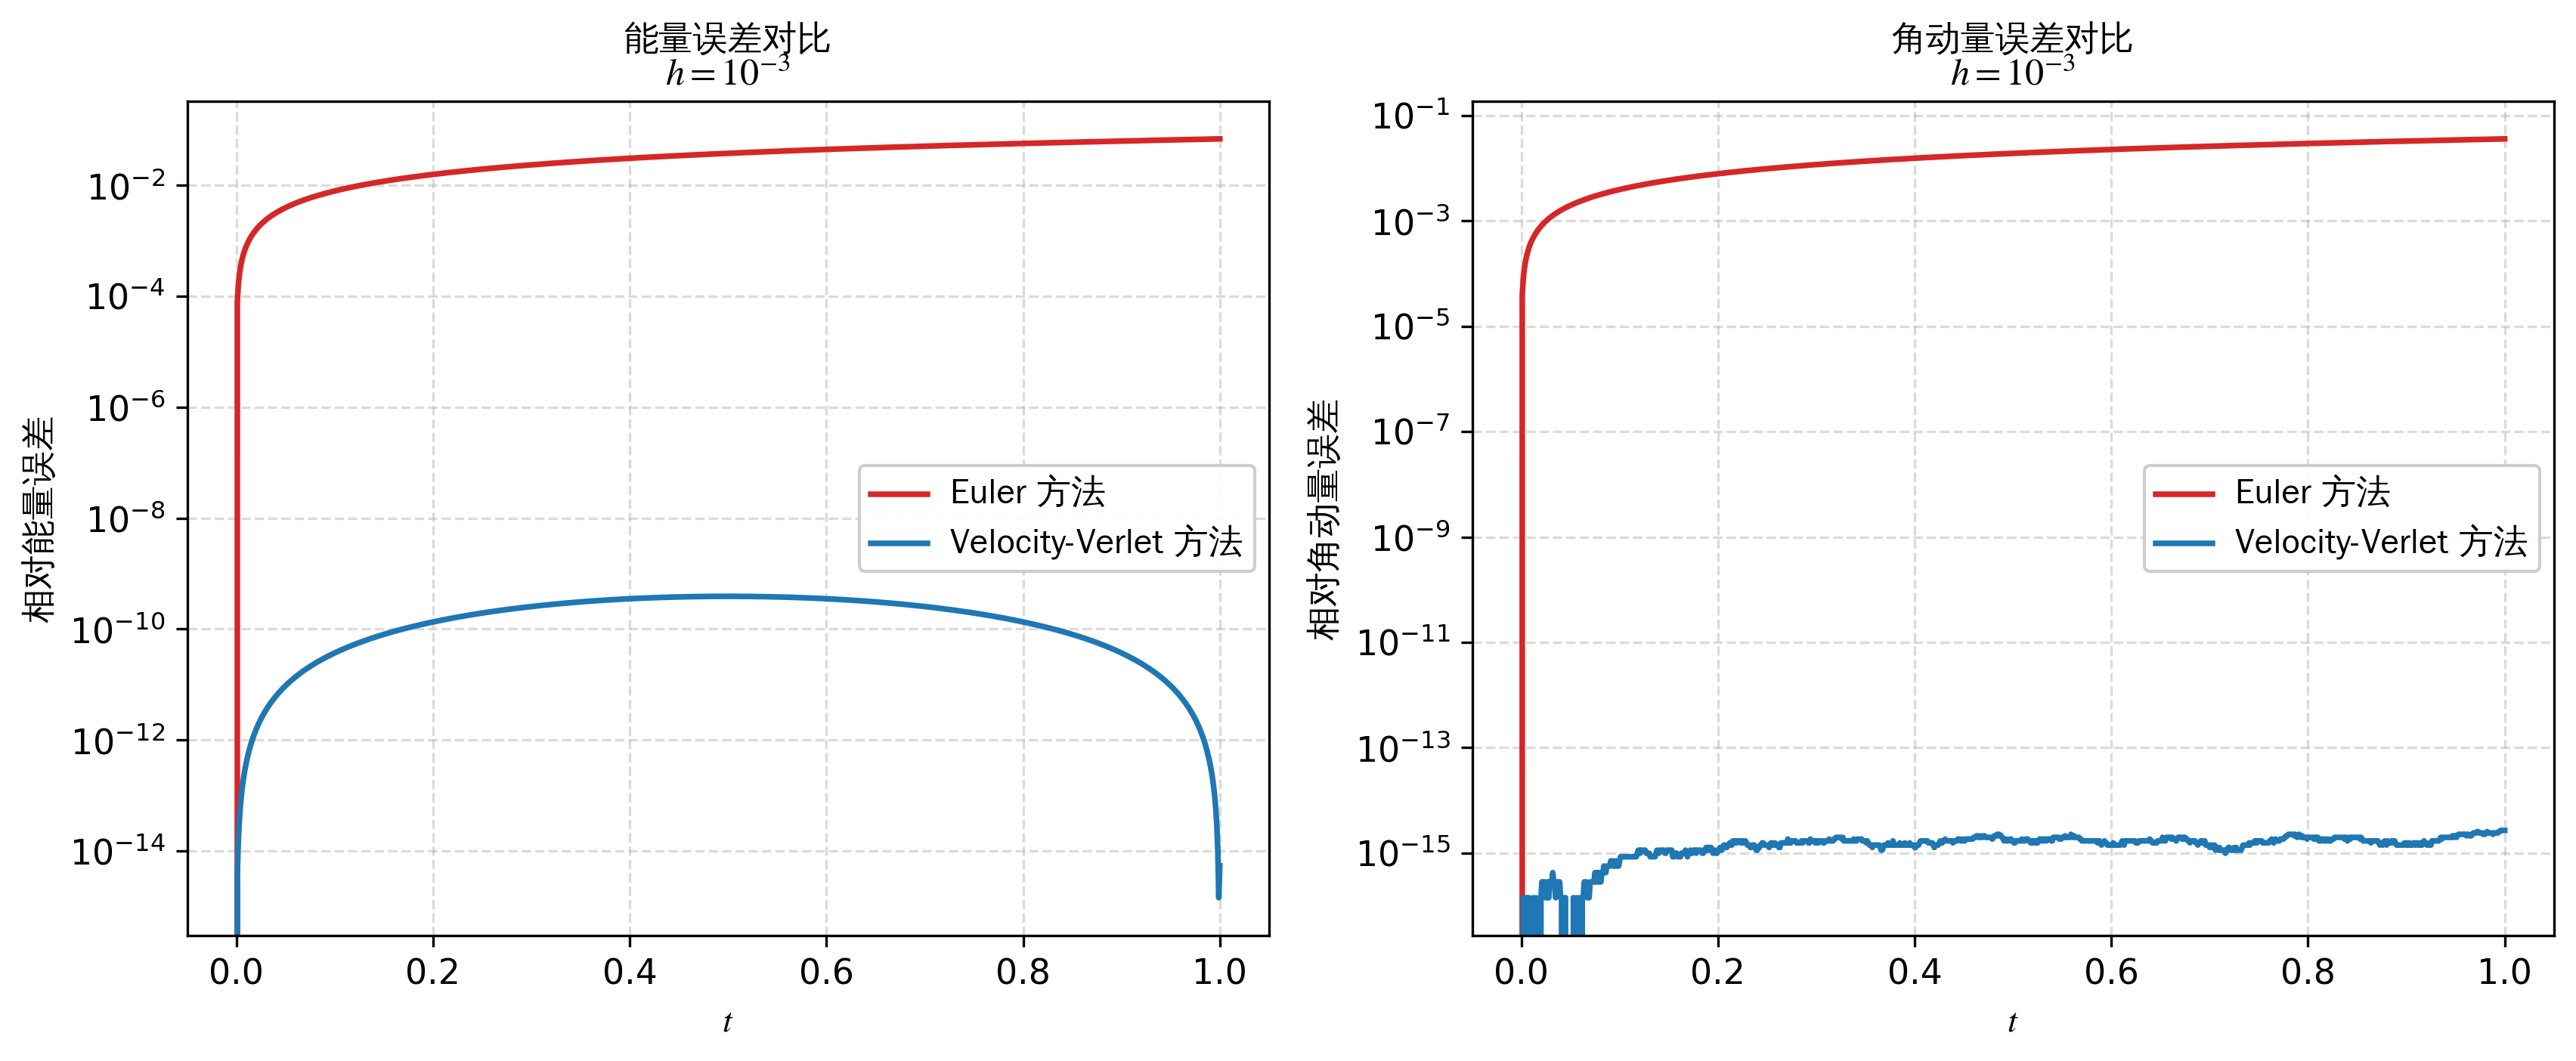
\includegraphics[width=0.92\textwidth]{images/conservation_errors_h1e-03.png}
\caption{步长 \(h=10^{-3}\) 时的守恒量误差对比。左图为相对能量误差，右图为相对角动量误差。与 \(h=10^{-2}\) 的情形相比，减小步长后两种方法的误差都进一步降低；但仍可明显看出，Euler 方法存在较显著的误差积累，而 Velocity-Verlet 方法的误差始终维持在接近机器精度的水平，反映出其在圆轨道长期传播中的优越表现。}
\label{fig:conservation-errors-h1e-3}
\end{figure}

从图 \ref{fig:circle-orbit-comparison} 可以直观看出，在圆轨道初值下，两种数值方法的表现存在明显差异。当步长取为 \(h=10^{-2}\) 时，Euler 方法得到的轨道已经明显偏离理论圆轨道，出现了较强的外扩漂移；相比之下，Velocity-Verlet 方法得到的轨道仍与理论圆轨道几乎重合，说明其在相同步长下具有更好的几何稳定性。当步长减小到 \(h=10^{-3}\) 时，Euler 方法的轨道误差虽然有所减小，但仍能观察到明显偏离；而 Velocity-Verlet 方法则继续保持了与理论圆轨道高度一致的数值结果。

这种差异在守恒量误差图中表现得更加清楚。由图 \ref{fig:conservation-errors-h1e-2} 可见，在较大步长 \(h=10^{-2}\) 下，Euler 方法的相对能量误差和相对角动量误差都随时间迅速增长，说明该方法在长期传播中会持续破坏系统的守恒结构；而 Velocity-Verlet 方法的误差始终维持在极小量级，表现出显著更好的稳定性。进一步地，从图 \ref{fig:conservation-errors-h1e-3} 可以看到，当步长减小到 \(h=10^{-3}\) 时，两种方法的误差都降低了，但 Euler 方法仍然存在明显的误差累积趋势，而 Velocity-Verlet 方法的能量误差与角动量误差依旧保持在接近机器精度的范围内。

综合这三张图可以得出结论：对于本文所研究的圆轨道保守系统，Euler 方法虽然实现最为简单，但数值耗散（或增益）效应较明显，难以在较长时间传播中保持轨道结构与守恒量；Velocity-Verlet 方法则能够在较低计算复杂度下更好地保持轨道几何形状，并有效控制能量与角动量误差，因此更适合作为本文后续日地系统数值模拟的基础方法。


\section{三维模型的推广}

\subsection{三维相对运动方程}

在三维情形下\cite{MurrayDermott1999,BateMuellerWhite1971}，取
\[
\bm r(t)=(x(t),y(t),z(t)),
\qquad
\bm v(t)=(v_x(t),v_y(t),v_z(t)).
\]
则相对运动方程为
\[
\ddot{\bm r}=-\mu \frac{\bm r}{\|\bm r\|^3},
\qquad
\|\bm r\|=\sqrt{x^2+y^2+z^2}.
\]
对应的一阶系统为
\[
\dot x=v_x,\quad \dot y=v_y,\quad \dot z=v_z,
\]
\[
\dot v_x=-\mu \frac{x}{(x^2+y^2+z^2)^{3/2}},\qquad
\dot v_y=-\mu \frac{y}{(x^2+y^2+z^2)^{3/2}},\qquad
\dot v_z=-\mu \frac{z}{(x^2+y^2+z^2)^{3/2}}.
\]

\subsection{三维模拟的意义}

从理论上说，二体问题总是限制在某个平面内，因此三维模型并不比二维更“本质复杂”；
但三维模拟仍然很有意义，因为它能够：
\begin{enumerate}[label=\arabic*.]
  \item 显式处理轨道倾角；
  \item 便于与 JPL 提供的三维状态向量直接对接\cite{JPLHorizonsManual}；
  \item 为以后加入摄动、多体效应和坐标变换做准备。
\end{enumerate}

例如，可取
\[
\bm r(0)=(1,0,0),
\qquad
\bm v(0)=\left(0,2\pi\cos i,2\pi\sin i\right),
\]
其中 \(i\) 为给定倾角。这样得到的轨道不再落在 \(xy\)-平面中，而是位于一个倾斜的轨道平面内。

\subsection{三维下的守恒量}

三维情形下的机械能仍为\cite{MurrayDermott1999}
\[
E=\frac12\|\bm v\|^2-\frac{\mu}{\|\bm r\|},
\]
角动量变为向量
\[
\bm L=\bm r\times \bm v.
\]
因此数值模拟时，除观察 \(E\) 是否近似守恒外，还应检查 \(\bm L\) 的模长及其方向是否近似不变。

\subsection{三维下的 Velocity-Verlet}

Velocity-Verlet 在三维中的形式与二维完全平行：
\[
\bm a(\bm r)=-\mu \frac{\bm r}{\|\bm r\|^3},
\]
\[
\bm a_n=\bm a(\bm r_n),
\]
\[
\bm r_{n+1}=\bm r_n+h\bm v_n+\frac{h^2}{2}\bm a_n,
\]
\[
\bm a_{n+1}=\bm a(\bm r_{n+1}),
\]
\[
\bm v_{n+1}=\bm v_n+\frac{h}{2}(\bm a_n+\bm a_{n+1}).
\]
因此程序结构几乎无需改变，只需把二维向量升级为三维向量即可\cite{HairerLubichWanner2006,LeimkuhlerReich2004}。

\section{实际太阳--地月系质心系统的模拟与 JPL 数据对比}

\subsection{为何选择 Sun--EM Bary 作为比较对象}

为了把简单的二体模型和真实天体数据联系起来，最自然的比较对象不是“太阳--地球中心”，而是“太阳--地月系质心（Sun--EM Bary）”。原因是：真实的地球会受到月球影响而围绕地月系质心摆动，而 JPL 在行星近似位置表和 Horizons 系统中都把 Earth--Moon Barycenter 作为标准对象之一。这样做既更接近真实太阳系动力学，也更便于调用官方星历数据。

为避免记号混淆，本节将“实际系统”理解为太阳与地月系质心之间的相对运动\cite{JPLHorizonsManual,JPLApproximatePositions}。其引力参数取为
\[
\mu_{\mathrm{SEMB}}=GM_{\odot}+GM_{\oplus}+GM_{\mathrm{Moon}}.
\]

\subsection{与 JPL Horizons 对接的基本思路}

JPL Horizons 可以输出某一天体相对于另一参考中心的笛卡尔状态向量或振荡轨道要素。
对于 Sun--EM Bary 系统，可令目标体为 Earth--Moon Barycenter，参考中心为 Sun，
然后获取某个历元的状态向量\cite{JPLHorizonsManual,JPLHorizonsAPI}
\[
\bm r_0=(x_0,y_0,z_0),
\qquad
\bm v_0=(v_{x,0},v_{y,0},v_{z,0}).
\]
然后：
\begin{enumerate}[label=\arabic*.]
  \item 在三维二体模型中，以 \((\bm r_0,\bm v_0)\) 作为初值进行积分；
  \item 若要得到二维模型，则把该状态向量投影到选定参考平面（通常取黄道平面）；
  \item 在后续时刻 \(t_n\) 上，把数值解 \((\bm r_n,\bm v_n)\) 与 Horizons 给出的参考状态作比较。
\end{enumerate}

设计实验比较以下几个量：

\begin{enumerate}[label=\arabic*.]
  \item 位置误差
  \[
  \varepsilon_r(t_n)=\|\bm r_{\mathrm{num}}(t_n)-\bm r_{\mathrm{JPL}}(t_n)\|;
  \]
  \item 速度误差
  \[
  \varepsilon_v(t_n)=\|\bm v_{\mathrm{num}}(t_n)-\bm v_{\mathrm{JPL}}(t_n)\|;
  \]
  \item 若只比较二维投影，还可比较平面角位置误差
  \[
  \varepsilon_\lambda(t_n)=|\lambda_{\mathrm{num}}(t_n)-\lambda_{\mathrm{JPL}}(t_n)|;
  \]
  \item 对于径向变化明显的情形，还可比较日距误差
  \[
  \varepsilon_\rho(t_n)=\left|\,\|\bm r_{\mathrm{num}}(t_n)\|-\|\bm r_{\mathrm{JPL}}(t_n)\|\right|.
  \]
\end{enumerate}

需要指出的是：二维相对运动模型本质上是一个固定平面内的二体模型，而 JPL Horizons 背后使用的是高精度太阳系星历。因此，两者即使在同一历元有相同初值，后续传播也不会严格重合。差异主要来自：
\begin{enumerate}[label=\arabic*.]
  \item 真实太阳系是多体系统，而不是严格二体系统；
  \item 真实轨道并不永远限制在一个固定平面内；
  \item JPL 参考解中包含了更完整的动力学与星历拟合信息。
\end{enumerate}

因此，二维模型与 JPL 的比较，更适合被理解为：
\begin{center}
一个教学级二体模型，对真实 Sun--EM Bary 运动的主轨道形状、主频率和短期相位的近似能力检验。
\end{center}

\subsection{一个可执行的对比实验}

下面给出一个基于真实 JPL Horizons 数据的三维对比实验。
比较对象取太阳--地月系质心系统（Sun--EM Bary），引力参数取为
\[
\mu_{\mathrm{SEMB}} = GM_\odot + GM_\oplus + GM_{\mathrm{Moon}},
\]
其中
\[
GM_\odot = 1.32712440041279419\times 10^{11}\ \mathrm{km^3\,s^{-2}},
\]
\[
GM_\oplus = 398600.435507\ \mathrm{km^3\,s^{-2}},
\qquad
GM_{\mathrm{Moon}} = 4902.800118\ \mathrm{km^3\,s^{-2}}.
\]
因此
\[
GM_{\mathrm{EMB}} = GM_\oplus + GM_{\mathrm{Moon}} = 403503.235625\ \mathrm{km^3\,s^{-2}},
\]
并有
\[
\mu_{\mathrm{SEMB}} = GM_\odot + GM_{\mathrm{EMB}}.
\]

实验中，选取参考历元 \(2026\text{-}01\text{-}01\) 的 TDB 时刻，从 JPL Horizons 获取 Earth--Moon Barycenter 相对 Sun 的三维状态向量
\[
\bm r_0=(x_0,y_0,z_0),\qquad
\bm v_0=(v_{x,0},v_{y,0},v_{z,0}),
\]
并将其作为三维二体模型的初值。计算得到该初值的量级约为
\[
\|\bm r_0\| \approx 1.471072\times 10^8\ \mathrm{km},
\qquad
\|\bm v_0\| \approx 3.028485\times 10^1\ \mathrm{km/s},
\]
这与真实日心轨道的尺度是一致的。随后，在三维二体模型
\[
\ddot{\bm r}
=
-\mu_{\mathrm{SEMB}}\frac{\bm r}{\|\bm r\|^3}
\]
下，采用 Velocity-Verlet 方法进行一年期传播。为保证传播精度，数值积分内部步长取为 \(3600\ \mathrm{s}\)，而与 JPL 参考解的比较则按每天一次的频率进行。

按照第 2.7.4 节的误差设计，定义位置误差、速度误差与日距误差分别为
\[
\varepsilon_r(t_n)=\|\bm r_{\mathrm{num}}(t_n)-\bm r_{\mathrm{JPL}}(t_n)\|,
\]
\[
\varepsilon_v(t_n)=\|\bm v_{\mathrm{num}}(t_n)-\bm v_{\mathrm{JPL}}(t_n)\|,
\]
\[
\varepsilon_\rho(t_n)=\bigl|\|\bm r_{\mathrm{num}}(t_n)\|-\|\bm r_{\mathrm{JPL}}(t_n)\|\bigr|.
\]
进一步地，为便于比较不同量纲量的相对偏差，再定义位置相对误差、速度相对误差与日距相对误差为
\[
\varepsilon_r^{\mathrm{rel}}(t_n)
=
\frac{\|\bm r_{\mathrm{num}}(t_n)-\bm r_{\mathrm{JPL}}(t_n)\|}{\|\bm r_{\mathrm{JPL}}(t_n)\|},
\]
\[
\varepsilon_v^{\mathrm{rel}}(t_n)
=
\frac{\|\bm v_{\mathrm{num}}(t_n)-\bm v_{\mathrm{JPL}}(t_n)\|}{\|\bm v_{\mathrm{JPL}}(t_n)\|},
\]
\[
\varepsilon_\rho^{\mathrm{rel}}(t_n)
=
\frac{\bigl|\|\bm r_{\mathrm{num}}(t_n)\|-\|\bm r_{\mathrm{JPL}}(t_n)\|\bigr|}{\|\bm r_{\mathrm{JPL}}(t_n)\|}.
\]

本次实验的误差统计结果如下：在一年传播区间内，位置绝对误差的最大值约为
\[
\max \varepsilon_r \approx 5.829\times 10^3\ \mathrm{km},
\]
其最大相对误差约为
\[
\max \varepsilon_r^{\mathrm{rel}} \approx 3.851\times 10^{-5}.
\]
速度绝对误差的最大值约为
\[
\max \varepsilon_v \approx 1.694\times 10^{-3}\ \mathrm{km/s},
\]
其最大相对误差约为
\[
\max \varepsilon_v^{\mathrm{rel}} \approx 5.593\times 10^{-5}.
\]
同时，日距绝对误差的最大值约为
\[
\max \varepsilon_\rho \approx 2.874\times 10^3\ \mathrm{km},
\]
其最大相对误差约为
\[
\max \varepsilon_\rho^{\mathrm{rel}} \approx 1.953\times 10^{-5}.
\]
在传播终点（约一年后），位置绝对误差约为
\[
\varepsilon_r(T)\approx 4.769\times 10^3\ \mathrm{km},
\]
速度绝对误差约为
\[
\varepsilon_v(T)\approx 1.694\times 10^{-3}\ \mathrm{km/s},
\]
而日距绝对误差约为
\[
\varepsilon_\rho(T)\approx 2.874\times 10^3\ \mathrm{km}.
\]

图 \ref{fig:sun-embary-jpl-errors} 给出了这一实验中的误差曲线。可以看到，位置误差与速度误差都没有表现出单调爆炸式增长，而是在全年传播中呈现出较为平滑的周期性起伏。这说明在当前实验设置下，三维二体模型与 JPL 参考解之间的差异，主要体现为轨道相位和轨道几何的缓慢偏离，而不是数值方法本身的失稳。特别地，在前几天的传播中，位置误差仍保持在个位数公里量级，这表明三维二体模型在短期内与高精度参考解具有非常好的吻合程度；随着传播时间增加，误差逐渐累积，并在年中达到较大值，但总体仍控制在 \(10^4\ \mathrm{km}\) 以内。

综合上述结果可以认为：对于 Sun--EM Bary 这一真实对象，尽管三维二体模型忽略了真实太阳系中的多体摄动、轨道平面缓慢变化以及更复杂的动力学修正，但它仍然能够在一年尺度内较好地复现真实轨道的主结构与主频率，并把位置误差控制在 \(10^4\ \mathrm{km}\) 以内、速度误差控制在 \(10^{-3}\ \mathrm{km/s}\) 量级。这说明三维二体模型已经能够作为一个有效的教学级近似模型，用于理解真实 Sun--EM Bary 轨道的主导动力学特征；与此同时，这一结果也表明，如果希望进一步缩小与 JPL 高精度星历之间的差异，则需要在当前模型基础上继续引入多体摄动或更高精度的动力学修正。

\begin{figure}[H]
\centering
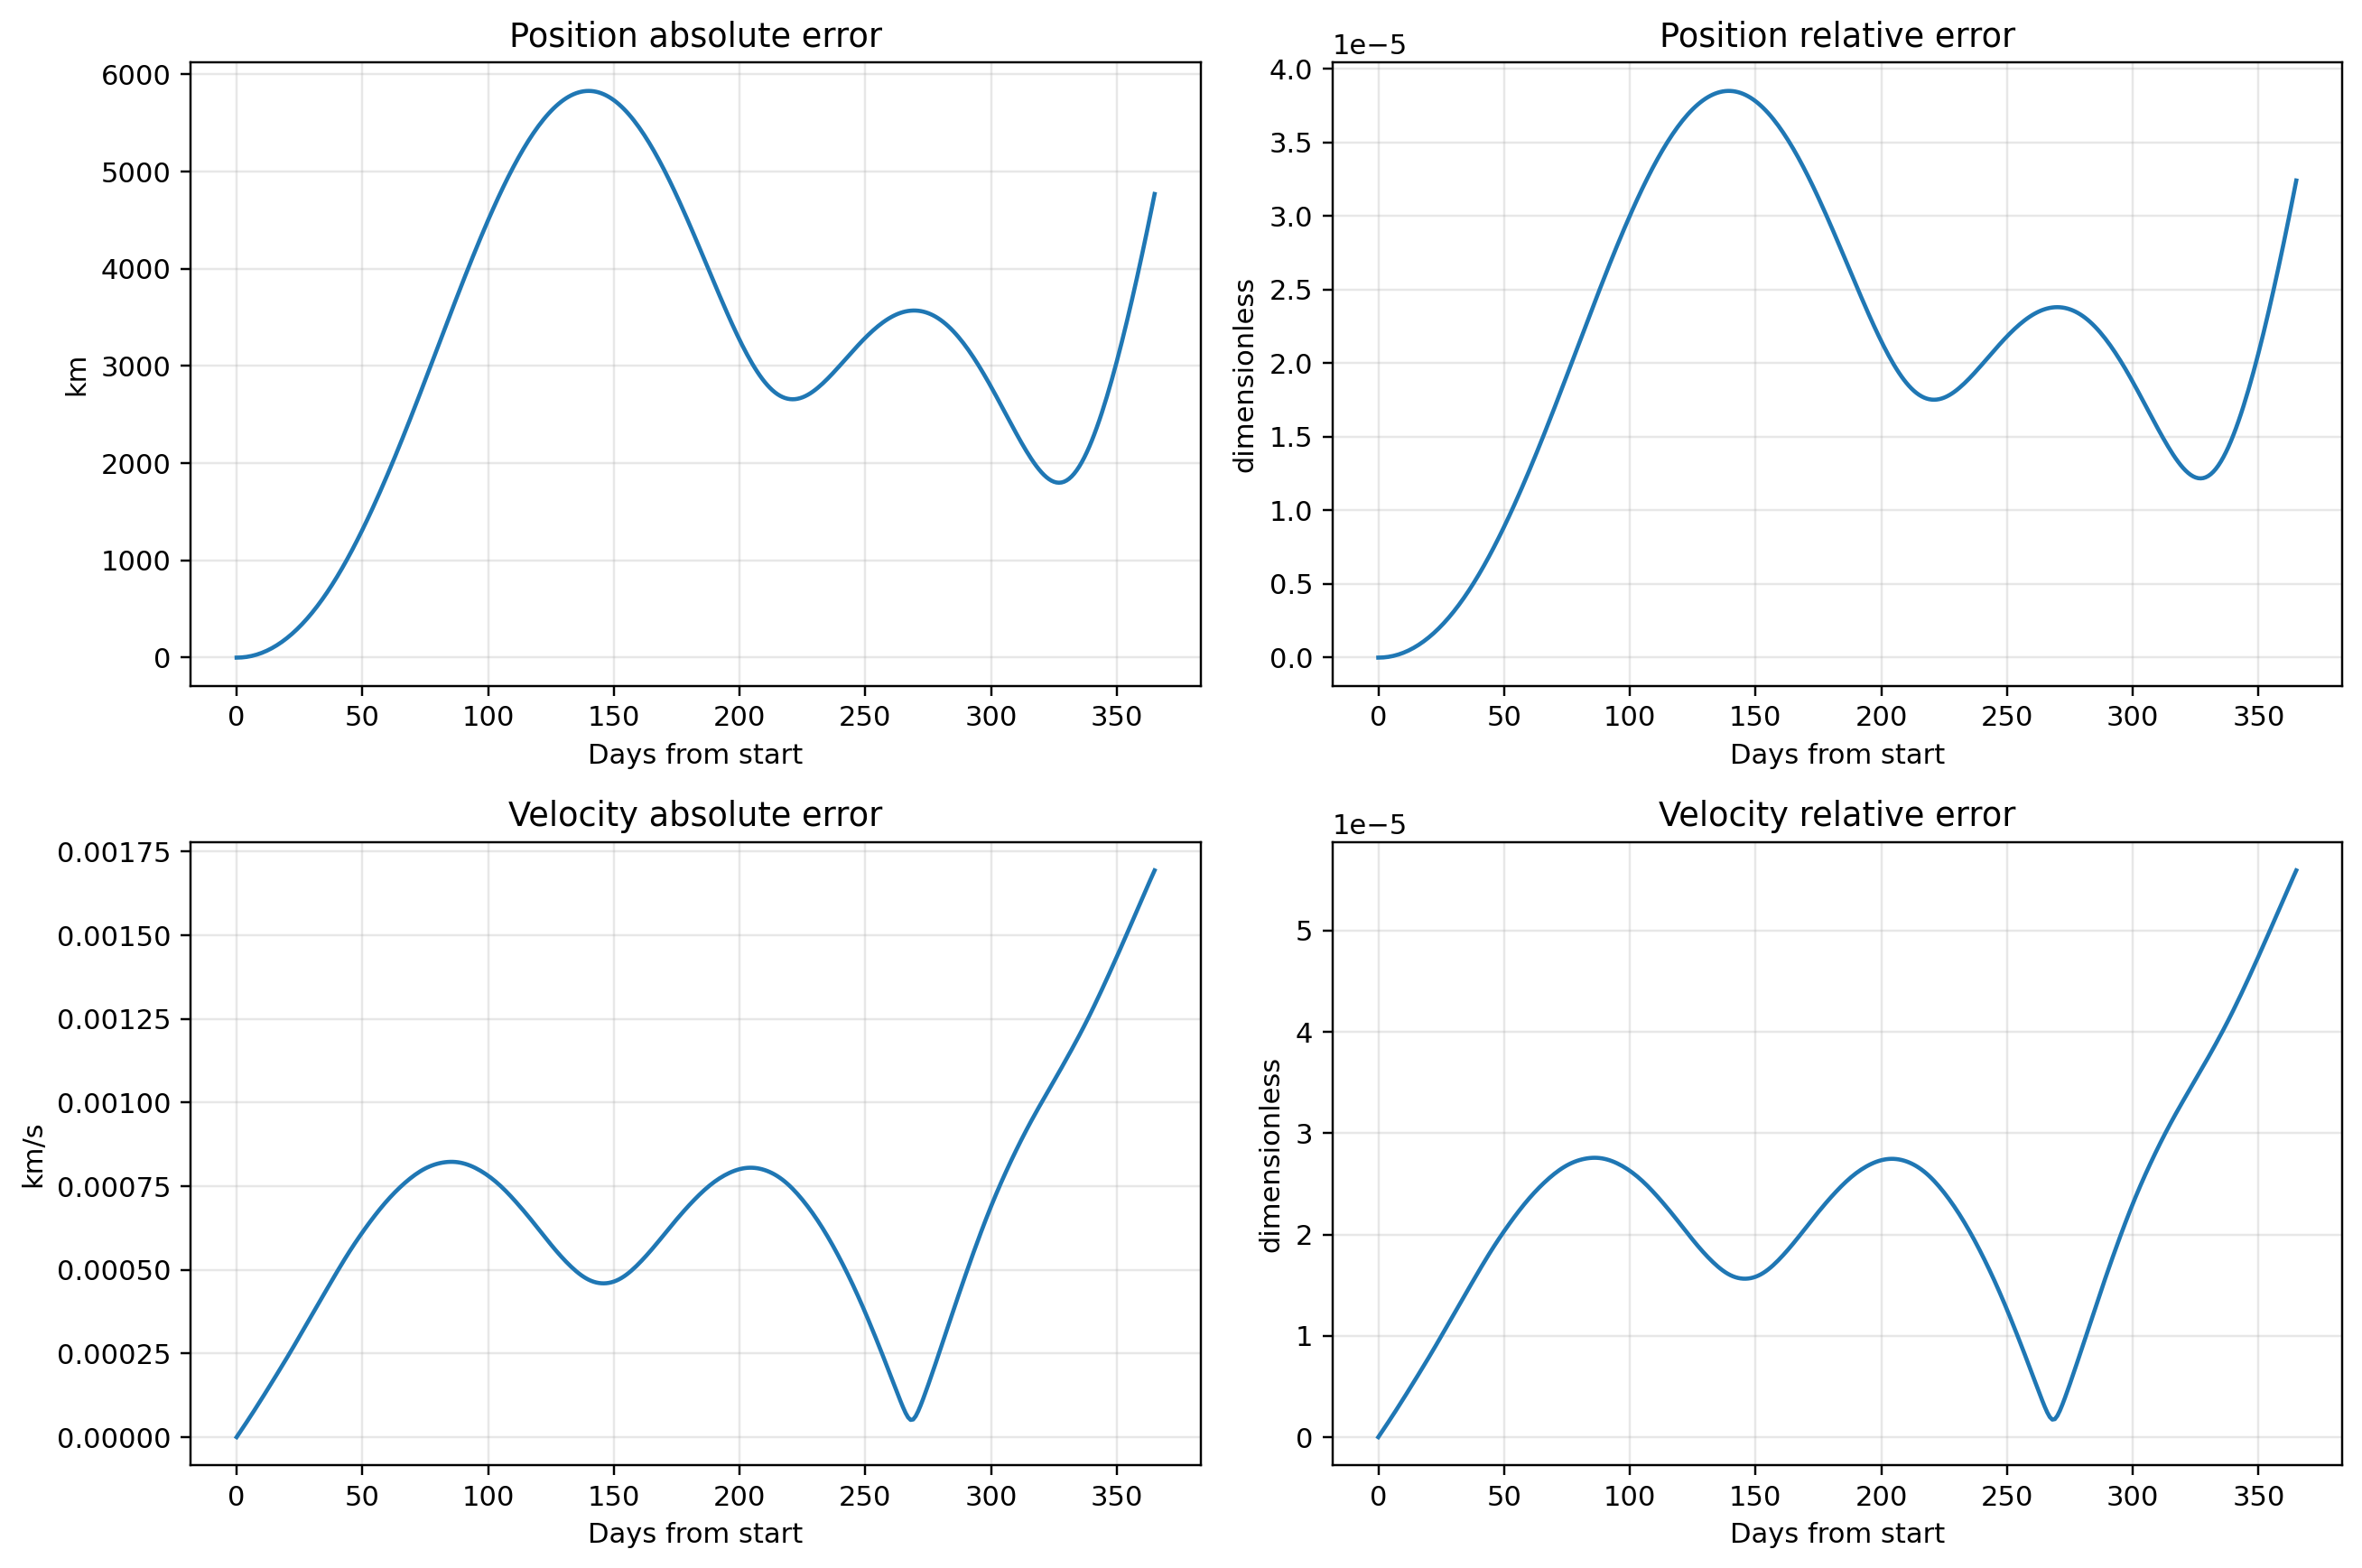
\includegraphics[width=0.95\textwidth]{jpl_compare_output/sun_embary_compare_errors.png}
\caption{Sun--EM Bary 三维二体模型与 JPL Horizons 参考解的误差对比。左上图为位置绝对误差，右上图为位置相对误差，左下图为速度绝对误差，右下图为速度相对误差。可以看到，在一年传播区间内，位置误差整体保持在 \(10^4\ \mathrm{km}\) 以内，速度误差保持在 \(10^{-3}\ \mathrm{km/s}\) 量级；误差曲线呈现明显的周期性起伏，而不是单调爆炸，说明三维二体模型能够较好地捕捉真实 Sun--EM Bary 轨道的主运动特征，但与 JPL 高精度多体星历之间仍存在可观测的系统性偏差。}
\label{fig:sun-embary-jpl-errors}
\end{figure}

\subsection{与 JPL 近似轨道要素的关系}

若不直接使用 Horizons 的向量表，也可先用 JPL 给出的 EM Bary 近似 Kepler 轨道要素作初值近似，然后再与 Horizons 精细数据比较。这样做的逻辑是：
\begin{enumerate}[label=\arabic*.]
  \item 用 JPL 的近似要素给出一个合理的初始椭圆轨道；
  \item 用二体模型数值传播得到轨道；
  \item 用 Horizons 作为高精度参考，检验二体模型在短期和中期内的误差累积。
\end{enumerate}
这比“随意给一个单位圆初值”更接近真实太阳系数据。

